\subsection{Frekvens Domænet}
Indtil nu har vi håndteret billederne i det spatiale domæne. I frekvens domænet arbejder vi med den rate hvormed pixel-værdierne ændre sig.\\

Det kan ofte være hurtigst at gå over i frekvens domænet, lave filter multiply for så at gå tilbage til det spatiale domæne, end det ville være at lave convolution i det spatiale donæme. 

\begin{figure}[H]
	\centering
	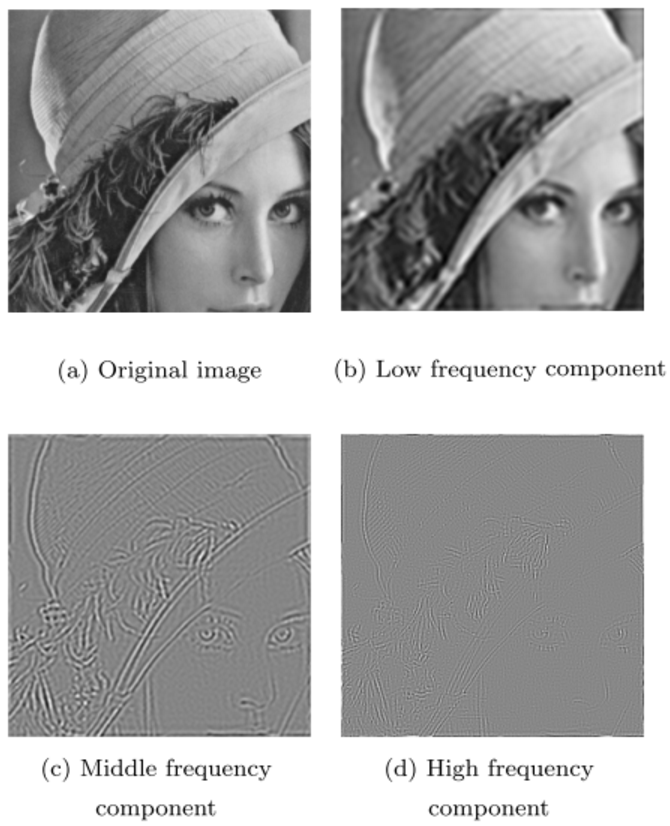
\includegraphics[width=0.7\linewidth]{figs/spm05/frequencies}
	\caption{Illustration af de forskellige frekvenser i et billede.}
	\label{fig:frequencies}
\end{figure}

Figur~\ref{fig:frequencies} viser hvor og hvordan de forskellige frekvenser optræder i et billede.\\

Som Figur~\ref{fig:frequencies} også viser så det de høje frekvenser vist i de hurtige ændringer, eksempelvis kanterne, og de lave frekvenser er de langsomme ændringer, overfladerne etc.